\documentclass[aspectratio=169]{beamer}

\usetheme{metropolis}

\usepackage{amsmath,amssymb}
\usepackage{graphicx}
\usepackage{booktabs}
\usepackage{array}
\usepackage{listings}
\usepackage{xcolor}
\usepackage{tikz}
\usetikzlibrary{arrows.meta,positioning}
\usepackage{qrcode}

% Consistent notation
\newcommand{\E}{\mathbb{E}}
\DeclareMathOperator*{\argmin}{arg\,min}
\DeclareMathOperator*{\argmax}{arg\,max}

% ------------------------------------------------------------------
% Code listings: sober, projector-safe (bold keywords, grey comments)
% ------------------------------------------------------------------
\lstdefinelanguage{Julia}{
  morekeywords={function,end,return,for,in,do,const,using,include,if,else,elseif,
                while,struct,mutable,let,begin,import,module,true,false},
  sensitive=true,
  morecomment=[l]\#,
  morestring=[b]",
}
\lstdefinestyle{code}{
  basicstyle=\ttfamily\fontsize{7.4}{8.8}\selectfont,
  keywordstyle=\bfseries,
  commentstyle=\itshape\color{black!45},
  showstringspaces=false,
  columns=fullflexible,
  keepspaces=true,
  extendedchars=true,
  aboveskip=2pt,
  belowskip=2pt,
  literate={θ}{{$\theta$}}1 {ε}{{$\varepsilon$}}1 {σ}{{$\sigma$}}1 {μ}{{$\mu$}}1
           {²}{{$^2$}}1 {·}{{$\cdot$}}1 {ₖ}{{$_k$}}1,
}
\lstset{style=code,language=Julia}
\newcommand{\smallcode}{\ttfamily\fontsize{6.6}{7.9}\selectfont}

\title{Deep Adaptive Design of Experiments\\for Dynamical Systems}
\author{Arno Strouwen \enspace {\footnotesize PumasAI \textperiodcentered\ KU Leuven} \\[0.5em]
        Sebastian Miclu\c{t}a-C\^ampeanu \enspace {\footnotesize JuliaHub \textperiodcentered\ University of Bucharest}}
\date{JuliaCon 2026}

\begin{document}

% ------------------------------------------------------------------
% Title
% ------------------------------------------------------------------
\begin{frame}
  \titlepage
\end{frame}

% ==================================================================
% Part 1 -- the problem and the theory
% ==================================================================

% ------------------------------------------------------------------
% Slide: notation and goal
% ------------------------------------------------------------------
\begin{frame}{Notation and goal}
  \small
  \begin{itemize}\setlength{\itemsep}{0.3em}
    \item $\theta$: the unknown parameters.
    \item $u$: the design.
    \item $y$: the observations.
  \end{itemize}

  \vspace{0.4em}
  State of belief \emph{before} the experiment:
  \vspace{-0.3em}
  \[
    p(\theta) \qquad \text{the \textbf{prior}}
  \]

  After the experiment, Bayes' rule updates it:
  \vspace{-0.3em}
  \[
    p(\theta \mid y, u) = \frac{p(y \mid \theta, u)\,p(\theta)}
                               {\displaystyle\int p(y \mid \theta', u)\,p(\theta')\,d\theta'}
    \qquad \text{the \textbf{posterior}}
  \]

  \alert{Bayesian experimental design: choose $u$ to make the posterior as sharp as possible.}
\end{frame}

% ------------------------------------------------------------------
% Slide: the bioreactor, concretely
% ------------------------------------------------------------------
\begin{frame}{Concretely: a fed-batch bioreactor}
  \small
  \setlength{\abovedisplayskip}{2pt}\setlength{\belowdisplayskip}{2pt}%
  \begin{columns}[c]
  \begin{column}{0.55\textwidth}
    {\footnotesize
    \begin{align*}
      \dot C_s &= -\tfrac{\mu(C_s)}{Y_{xs}}\,C_x + \tfrac{Q_{\mathrm{in}}}{V}\,(C_{s,\mathrm{in}} - C_s),\\
      \dot C_x &= \mu(C_s)\,C_x - \tfrac{Q_{\mathrm{in}}}{V}\,C_x,\\
      \dot V   &= Q_{\mathrm{in}},
      \qquad \mu(C_s) = \frac{\mu_{\max}\,C_s}{K_s + C_s}.
    \end{align*}}
    \vspace{-0.2em}
    Substrate is pumped in, biomass eats it and grows, and the vessel fills up.
  \end{column}
  \begin{column}{0.42\textwidth}
    \begin{center}
    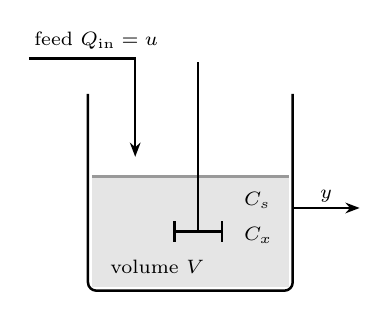
\begin{tikzpicture}[line width=0.9pt, every node/.style={font=\scriptsize}]
      % feed line, entering from the left
      \draw[-{Stealth[length=1.8mm]}] (-0.75,2.95) -- (0.6,2.95) -- (0.6,1.7);
      \node[anchor=south west, inner sep=1.5pt] at (-0.75,3.0) {feed $Q_{\mathrm{in}} = u$};
      % vessel, open top
      \draw[rounded corners=3pt] (0,2.5) -- (0,0) -- (2.6,0) -- (2.6,2.5);
      % liquid
      \fill[black!10] (0.05,0.05) rectangle (2.55,1.45);
      \draw[black!40] (0.05,1.45) -- (2.55,1.45);
      % impeller
      \draw (1.4,2.9) -- (1.4,0.75);
      \draw (1.1,0.75) -- (1.7,0.75);
      \draw (1.1,0.62) -- (1.1,0.88);
      \draw (1.7,0.62) -- (1.7,0.88);
      % contents
      \node[anchor=west] at (1.85,1.15) {$C_s$};
      \node[anchor=west] at (1.85,0.7) {$C_x$};
      \node[anchor=west] at (0.15,0.3) {volume $V$};
      % sample
      \draw[-{Stealth[length=1.8mm]}] (2.6,1.05) -- (3.45,1.05)
        node[midway,above,inner sep=1.5pt] {$y$};
    \end{tikzpicture}
    \end{center}
  \end{column}
  \end{columns}

  \begin{itemize}\setlength{\itemsep}{0.25em}
    \item \textbf{Design} $u = Q_{\mathrm{in}}$: the feed rate, which we may change once an hour.
    \item \textbf{Observations} $y = C_s + \text{noise}$: the substrate concentration, sampled once an hour.
    \item \textbf{Unknown} $\theta = (\mu_{\max}, K_s)$: the two constants in the growth law $\mu$.
  \end{itemize}

  \vspace{0.4em}
  \alert{Which feed profile makes the posterior over $\mu_{\max}$ and $K_s$ as sharp as possible?}
\end{frame}

% ------------------------------------------------------------------
% Slide: scoring a design
% ------------------------------------------------------------------
\begin{frame}{Scoring a design}
  \small
  \setlength{\abovedisplayskip}{2pt}\setlength{\belowdisplayskip}{2pt}%
  How sharp is a posterior? Measure it by its \textbf{entropy}, small when sharp and large when vague:
  \[
    H\big[p(\theta \mid y, u)\big] = -\int p(\theta \mid y, u)\,\log p(\theta \mid y, u)\, d\theta .
  \]

  $y$ is not measured yet, so we average over every observation the design could produce:
  \[
    u^\star = \argmin_u\ \E_{y \mid u}\big[\,H[p(\theta \mid y, u)]\,\big] .
  \]

  \vspace{0.5em}
  {\footnotesize \textbf{Technical note.}\ \ In our examples only part of $\theta$ is of interest:
  split $\theta = (\theta_T, \theta_N)$ into the kinetics $\theta_T$ and nuisance $\theta_N$
  (sensor noise, initial biomass), and score only the marginal posterior of the target,
  \[
    u^\star = \argmin_u\ \E_{y \mid u}\big[\,H[p(\theta_T \mid y, u)]\,\big],
    \qquad p(\theta_T \mid y, u) = \int p(\theta \mid y, u)\, d\theta_N .
  \]
  We will not go into what that does to the estimator here; it is in the paper:\\
  \emph{Deep Adaptive Model-Based Design of Experiments}, arXiv:2603.16146.}
\end{frame}

% ------------------------------------------------------------------
% Slide: why it is expensive
% ------------------------------------------------------------------
\begin{frame}{Why that is expensive}
  \small
  \setlength{\abovedisplayskip}{1pt}\setlength{\belowdisplayskip}{1pt}%
  Up to a constant, the entropy criterion can be rewritten as
  \[
    \max_u\ \E_{\theta,\, y \mid u}\big[\log p(y \mid \theta, u) - \log p(y \mid u)\big].
  \]
  The first term is easy: simulate the model and evaluate its likelihood.

  The second term is the \textbf{evidence}, an integral over every parameter the prior allows:
  \[
    p(y \mid u) = \int p(y \mid \theta, u)\,p(\theta)\,d\theta .
  \]
  Replace it by a sample average and you get a loop inside a loop:
  \[
    \frac{1}{N}\sum_{n=1}^{N}\Big[
      \log p\big(y_n \mid \theta^{(n)}, u\big)
      \;-\; \log \underbrace{\frac{1}{L}\sum_{\ell=1}^{L} p\big(y_n \mid \theta^{(\ell)}, u\big)}_{\text{inner loop}}
    \Big]
  \]
  Every one of those likelihoods is an ODE solve.

  \alert{$N \times L$ ODE solves to score \emph{one} candidate design, and the optimizer wants many.}

\end{frame}

% ------------------------------------------------------------------
% Slide: static, adaptive, policies
% ------------------------------------------------------------------
\begin{frame}{From static schedules to policies}
  \small
  \setlength{\abovedisplayskip}{1pt}\setlength{\belowdisplayskip}{1pt}%
  \textbf{Static:} choose the whole input sequence $u_{1:K} = (u_1, \dots, u_K)$ before the experiment.

  \vspace{0.35em}
  \textbf{Adaptive:} choose $u_k$ only after seeing the history
  $h_{k-1} = (u_1, y_1, \dots, u_{k-1}, y_{k-1})$ of all inputs and measurements so far.
  The optimum alternates a decision and an expectation at every step:
  \[
    V = \min_{u_1}\E_{y_1}\min_{u_2}\E_{y_2}\cdots\min_{u_K}\E_{y_K}
        \big[\,H[p(\theta \mid h_K)]\,\big].
  \]
  The usual workaround: after each measurement, update the posterior and re-optimize only the next
  input --- inference and optimization, between two measurements.

  \vspace{0.35em}
  \textbf{Instead:} optimize over the rules themselves: a \textbf{policy} $\pi$ maps history to
  next input, $u_k = \pi(h_{k-1})$. Over that function space the nesting collapses exactly into
  one expectation:
  \[
    V = \min_{\pi}\ \E_{h_K \mid \pi}\big[\,H[p(\theta \mid h_K)]\,\big].
  \]
  A neural network $\pi_\phi$ is just an approximation of that space, trained by policy gradient
  on simulated episodes.

  \vspace{0.35em}
  \alert{Trained once, offline; in the lab, each step is one forward pass.}
\end{frame}

% ------------------------------------------------------------------
% Slide: cost of one gradient step
% ------------------------------------------------------------------
\begin{frame}{What one gradient step costs}
  \small
  \setlength{\abovedisplayskip}{4pt}\setlength{\belowdisplayskip}{4pt}%
  Scoring one episode means re-simulating it under hundreds of parameter draws from the prior.
  That is $932$ ODE solves per episode, and training scores a batch of $53{,}648$ episodes:
  \[
    \underbrace{932}_{\text{per episode}} \times \underbrace{53{,}648}_{\text{episodes}}
    \approx 5 \times 10^{7} \ \text{ODE solves}.
  \]
  And training needs the \emph{gradient} of that whole computation at every optimizer step,
  not just its value. Even done well, one gradient step takes $15.4$\,s on an H100.

  \vspace{0.7em}
  \alert{So the batch has to live on the GPU, the objective has to become one compiled program,
  and the solver has to be differentiated for us.}
\end{frame}

% ==================================================================
% Part 2 -- the Julia implementation
% ==================================================================

% ------------------------------------------------------------------
% Slide: the stack, as a compilation pipeline
% ------------------------------------------------------------------
\begin{frame}{The stack: from Julia code to one GPU executable}
  \small
  \begin{center}
  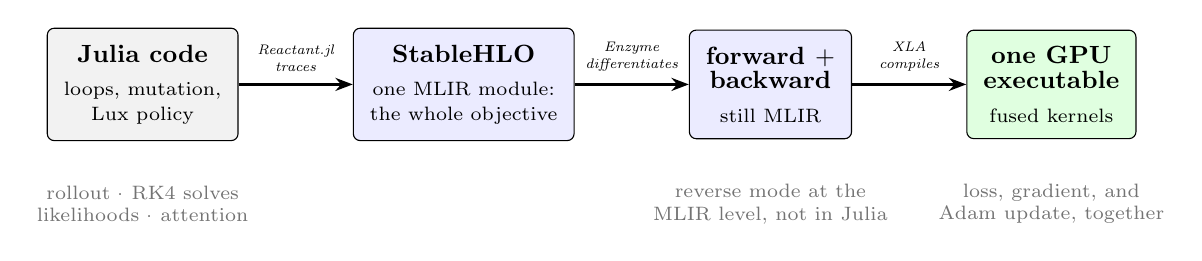
\begin{tikzpicture}[
      box/.style={draw, rounded corners=2.5pt, align=center, inner sep=6pt,
                  minimum height=1.15cm, font=\small},
      sub/.style={font=\scriptsize, color=black!55, align=center},
      lbl/.style={font=\tiny\itshape, align=center},
      arr/.style={-{Stealth[length=2.2mm]}, line width=1pt},
      node distance=1.45cm]
    \node[box, fill=black!5] (julia)
      {\textbf{Julia code}\\[1pt]{\scriptsize loops, mutation,}\\[-2pt]{\scriptsize Lux policy}};
    \node[box, right=of julia, fill=blue!8] (hlo)
      {\textbf{StableHLO}\\[1pt]{\scriptsize one MLIR module:}\\[-2pt]{\scriptsize the whole objective}};
    \node[box, right=of hlo, fill=blue!8] (grad)
      {\textbf{forward $+$}\\[-2pt]\textbf{backward}\\[1pt]{\scriptsize still MLIR}};
    \node[box, right=of grad, fill=green!12] (exe)
      {\textbf{one GPU}\\[-2pt]\textbf{executable}\\[1pt]{\scriptsize fused kernels}};
    \draw[arr] (julia) -- node[lbl, above=1pt] {Reactant.jl\\traces} (hlo);
    \draw[arr] (hlo)   -- node[lbl, above=1pt] {Enzyme\\differentiates} (grad);
    \draw[arr] (grad)  -- node[lbl, above=1pt] {XLA\\compiles} (exe);
    % what gets traced in
    \node[sub, below=0.45cm of julia] {rollout \textperiodcentered\ RK4 solves\\
                                       likelihoods \textperiodcentered\ attention};
    \node[sub, below=0.45cm of grad] {reverse mode at the\\MLIR level, not in Julia};
    \node[sub, below=0.45cm of exe] {loss, gradient, and\\Adam update, together};
  \end{tikzpicture}
  \end{center}

  \vspace{0.4em}
  {\footnotesize
  \begin{tabular}{@{}>{\raggedright\arraybackslash}p{0.30\textwidth}>{\raggedright\arraybackslash}p{0.30\textwidth}>{\raggedright\arraybackslash}p{0.32\textwidth}@{}}
    \textbf{Lux.jl}: weights are explicit arguments, so the loss is a pure function
    --- what a tracing compiler needs. &
    \textbf{SimpleDiffEq}: its RK4 \texttt{step!} drops into the traced loop unchanged. &
    \textbf{Optimisers.jl}: the update rides along via
    \texttt{Lux.Training.single\_train\_step!}. \\
  \end{tabular}}

  \vspace{0.4em}
  \alert{One gradient step becomes one compiled executable: no Julia left in the inner loop.}
\end{frame}

% ------------------------------------------------------------------
% Slide: the memory problem
% ------------------------------------------------------------------
\begin{frame}{The catch: reverse mode must remember the forward pass}
  \small
  To run the chain rule backwards, Enzyme needs the state at \emph{every} RK4 substep
  of every trajectory --- visited in reverse, after the forward pass is done.

  \begin{center}
  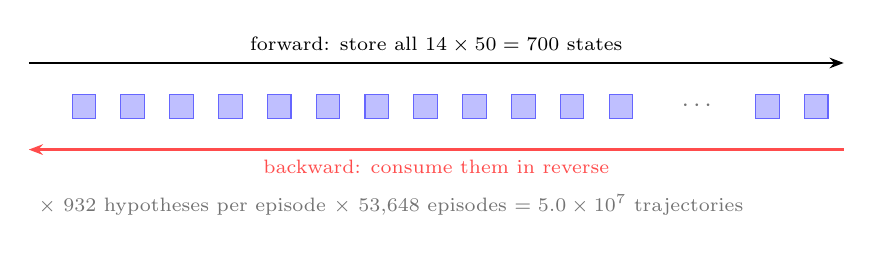
\begin{tikzpicture}[
      st/.style={draw=blue!60, fill=blue!25, minimum size=0.3cm, inner sep=0pt},
      arr/.style={-{Stealth[length=1.8mm]}, thick}]
    % forward chain of stored states
    \foreach \i in {0,...,11} {
      \node[st] (s\i) at (0.62*\i, 0) {};
    }
    \node[font=\small, color=black!55] at (0.62*12.6, 0) {$\cdots$};
    \foreach \i in {14,15} {
      \node[st] (s\i) at (0.62*\i, 0) {};
    }
    \draw[arr] (-0.7,0.55) -- node[above, font=\scriptsize] {forward: store all $14 \times 50 = 700$ states} (0.62*15+0.35,0.55);
    \draw[arr, red!70] (0.62*15+0.35,-0.55) -- node[below, font=\scriptsize] {backward: consume them in reverse} (-0.7,-0.55);
    \node[font=\scriptsize, color=black!55, anchor=west] at (-0.7, -1.25)
      {$\times\ 932$ hypotheses per episode $\times\ 53{,}648$ episodes $= 5.0 \times 10^{7}$ trajectories};
  \end{tikzpicture}
  \end{center}

  \vspace{0.3em}
  \setlength{\abovedisplayskip}{2pt}\setlength{\belowdisplayskip}{2pt}%
  \[
    \underbrace{3.5 \times 10^{10}}_{\text{stored states}} \times
    \underbrace{3}_{(C_s,\, C_x,\, V)} \times
    \underbrace{4\ \text{bytes}}_{\text{Float32}}
    \;\approx\; 420\ \text{GB} \qquad \text{--- and that is the state alone.}
  \]

  \begin{center}
  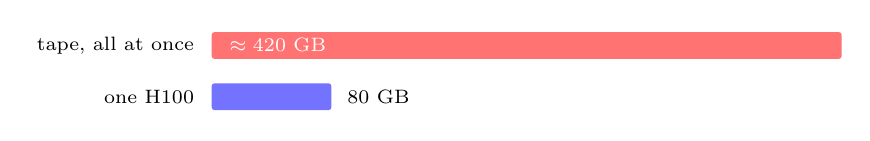
\begin{tikzpicture}[font=\scriptsize]
    % bars: 420 GB vs 80 GB, scale 8cm total
    \node[anchor=east] at (0, 0) {tape, all at once};
    \draw[fill=red!55, draw=none, rounded corners=1pt] (0.1, -0.17) rectangle (8.1, 0.17);
    \node[anchor=west, color=white] at (0.2, 0) {$\approx 420$ GB};
    \node[anchor=east] at (0, -0.65) {one H100};
    \draw[fill=blue!55, draw=none, rounded corners=1pt] (0.1, -0.82) rectangle (1.62, -0.48);
    \node[anchor=west] at (1.7, -0.65) {80 GB};
  \end{tikzpicture}
  \end{center}

  \alert{Naively, one gradient step needs $5\times$ the memory of the GPU --- before counting RK4 stages.}
\end{frame}

% ------------------------------------------------------------------
% Slide: first cut -- mini-batching / SGD
% ------------------------------------------------------------------
\begin{frame}[fragile]{First cut: the gradient is an expectation}
  \small
  \setlength{\abovedisplayskip}{2pt}\setlength{\belowdisplayskip}{2pt}%
  The objective is an expectation over simulated episodes; a sample average of gradients is
  \textbf{unbiased at any} $B$ --- batch size buys \emph{variance}, not correctness:
  \[
    \nabla_\phi \mathcal{L}
      = \E_{\theta \sim p(\theta),\, \varepsilon}\!\big[\nabla_\phi\, \ell(\phi;\theta,\varepsilon)\big]
      \;\approx\; \frac{1}{B}\sum_{b=1}^{B} \nabla_\phi\, \ell\big(\phi;\theta^{(b)}\!,\varepsilon^{(b)}\big).
  \]

  \vspace{0.1em}
  \begin{columns}[c]
  \begin{column}{0.42\textwidth}
    \begin{center}
    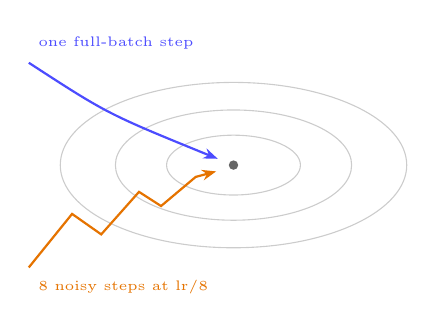
\begin{tikzpicture}[font=\tiny]
      \draw[black!20] (0,0) ellipse (2.2 and 1.05);
      \draw[black!20] (0,0) ellipse (1.5 and 0.7);
      \draw[black!20] (0,0) ellipse (0.85 and 0.38);
      \node[circle, fill=black!60, inner sep=1.2pt] at (0,0) {};
      % full-batch: one long smooth step
      \draw[-{Stealth[length=1.8mm]}, blue!70, thick]
        (-2.6,1.3) .. controls (-1.6,0.65) .. (-0.2,0.08);
      \node[color=blue!70, anchor=west] at (-2.6,1.55) {one full-batch step};
      % SGD zigzag
      \draw[-{Stealth[length=1.8mm]}, orange!90!black, thick]
        (-2.6,-1.3) -- (-2.05,-0.62) -- (-1.68,-0.88) -- (-1.2,-0.34)
        -- (-0.92,-0.52) -- (-0.48,-0.15) -- (-0.22,-0.08);
      \node[color=orange!90!black, anchor=west] at (-2.6,-1.55) {8 noisy steps at $\mathrm{lr}/8$};
    \end{tikzpicture}
    \end{center}
  \end{column}
  \begin{column}{0.54\textwidth}
    {\footnotesize Stochastic gradient descent, then: 8 strips of $6{,}706$ episodes, one Adam
    step per strip at $\mathrm{lr}/8$ --- an eighth of the activations alive at once.}
    \begin{center}
    
\begin{tikzpicture}[font=\tiny]
      \foreach \i/\c in {0/green!45, 1/green!45, 2/green!45, 3/blue!50, 4/black!12, 5/black!12, 6/black!12, 7/black!12} {
        \draw[fill=\c, draw=black!30, rounded corners=1pt]
          (0.62*\i, 0) rectangle (0.62*\i+0.54, 0.55);
      }
    \end{tikzpicture}
    \end{center}
\begin{lstlisting}
for _k in 1:8   # micro-batches; Adam at lr/8
    data = prepare_batch(rng, ...)  # fresh draws
    _, loss, _, ts = single_train_step!(
        AutoEnzyme(), spce_loss, data, ts)
end
\end{lstlisting}
  \end{column}
  \end{columns}

  \vspace{0.3em}
  \alert{And there is no dataset to shortchange: every strip is freshly simulated from the prior.}
\end{frame}

% ------------------------------------------------------------------
% Slide: second cut -- mincut rematerialization
% ------------------------------------------------------------------
\begin{frame}[fragile]{Second cut: checkpoint the substeps}
  \small
  A strip still stores all 50 RK4 states per control step. Enzyme's min-cut keeps
  ${\approx}\sqrt{N}$ of them; the backward pass recomputes the rest from the nearest
  checkpoint --- twice the forward FLOPs, a seventh of the memory.

  \begin{center}
  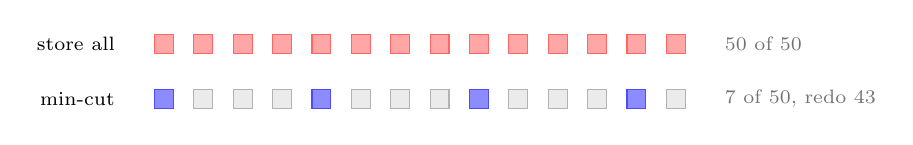
\begin{tikzpicture}[
      ck/.style={draw=blue!70, fill=blue!45, minimum size=0.24cm, inner sep=0pt},
      dr/.style={draw=black!30, fill=black!8, minimum size=0.24cm, inner sep=0pt},
      st/.style={draw=red!60, fill=red!35, minimum size=0.24cm, inner sep=0pt}]
    % naive row
    \node[font=\scriptsize, anchor=east] at (-0.5, 0) {store all};
    \foreach \i in {0,...,13} { \node[st] at (0.5*\i, 0) {}; }
    \node[font=\scriptsize, color=black!55, anchor=west] at (7.0, 0) {50 of 50};
    % mincut row
    \node[font=\scriptsize, anchor=east] at (-0.5, -0.7) {min-cut};
    \foreach \i/\s in {0/ck, 1/dr, 2/dr, 3/dr, 4/ck, 5/dr, 6/dr, 7/dr, 8/ck, 9/dr, 10/dr, 11/dr, 12/ck, 13/dr} {
      \node[\s] at (0.5*\i, -0.7) {};
    }
    \node[font=\scriptsize, color=black!55, anchor=west] at (7.0, -0.7) {7 of 50, redo 43};
  \end{tikzpicture}
  \end{center}

  \begin{columns}[c]
  \begin{column}{0.46\textwidth}
    \begin{center}
    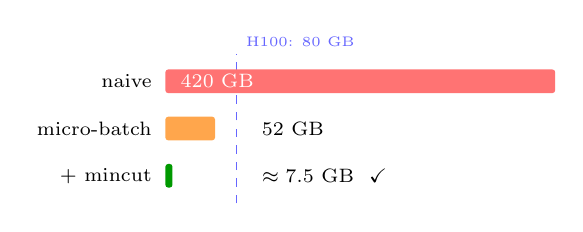
\begin{tikzpicture}[font=\scriptsize]
      % H100 reference line, drawn first so labels sit on top
      \draw[dashed, blue!60] (0.95, -1.55) -- (0.95, 0.35);
      \node[font=\tiny, color=blue!60, anchor=south west] at (0.95, 0.32) {H100: 80 GB};
      \node[anchor=east] at (0, 0) {naive};
      \draw[fill=red!55, draw=none, rounded corners=1pt] (0.05, -0.15) rectangle (5.0, 0.15);
      \node[anchor=west, color=white] at (0.12, 0) {420 GB};
      \node[anchor=east] at (0, -0.6) {micro-batch};
      \draw[fill=orange!70, draw=none, rounded corners=1pt] (0.05, -0.75) rectangle (0.68, -0.45);
      \node[anchor=west] at (1.15, -0.6) {52 GB};
      \node[anchor=east] at (0, -1.2) {$+$ mincut};
      \draw[fill=green!60!black, draw=none, rounded corners=1pt] (0.05, -1.35) rectangle (0.14, -1.05);
      \node[anchor=west] at (1.15, -1.2) {$\approx 7.5$ GB \ \checkmark};
    \end{tikzpicture}
    \end{center}
  \end{column}
  \begin{column}{0.50\textwidth}
    In the code, the entire plan is one annotation:
\begin{lstlisting}
@trace mincut=true for _ in 1:n_substeps
    u = rk4_step(u, θ, d, dt_sub)
end
\end{lstlisting}
  \end{column}
  \end{columns}

  \vspace{0.3em}
  \alert{No manual checkpoints, no custom backward pass --- memory becomes a tracing annotation.}
\end{frame}

% ------------------------------------------------------------------
% Slide: the policy in Lux
% ------------------------------------------------------------------
\begin{frame}[fragile]{The policy: a small transformer over the history}
\begin{lstlisting}
const policy = @compact(
    input_proj  = Dense(2 => 32),
    rms1 = RMSNorm((32,)),  mha = MultiHeadAttention(32; nheads = 4),
    rms2 = RMSNorm((32,)),  ff  = Chain(Dense(32 => 64, gelu), Dense(64 => 32)),
    output_head = Dense(32 => 1; init_bias = (rng, dims...) -> fill(-4.0f0, dims...)),
) do x                                        # x: (2, K, B) -- the (yₖ, uₖ) pairs so far
    x = input_proj(x)
    x = x .+ reshape(sinusoidal_pe(size(x, 2)), 32, :, 1)     # make time explicit
    attn, _ = mha(rms1(x))
    x = x + attn
    x = x + ff(rms2(x))
    @return ACTION_HI .* sigmoid.(output_head(x[:, end, :]))  # next feed rate in [0, 10]
end
\end{lstlisting}

  \vspace{0.2em}
  \begin{center}
  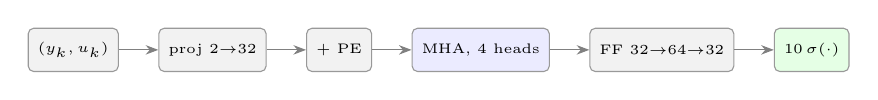
\begin{tikzpicture}[
      pb/.style={draw=black!40, rounded corners=2pt, fill=black!5, font=\tiny, align=center,
                 inner sep=3.5pt, minimum height=0.55cm},
      parr/.style={-{Stealth[length=1.6mm]}, black!50}]
    \node[pb] (a) {$(y_k, u_k)$};
    \node[pb, right=0.5cm of a] (b) {proj $2{\to}32$};
    \node[pb, right=0.5cm of b] (c) {$+$ PE};
    \node[pb, right=0.5cm of c, fill=blue!8] (d) {MHA, 4 heads};
    \node[pb, right=0.5cm of d] (e) {FF $32{\to}64{\to}32$};
    \node[pb, right=0.5cm of e, fill=green!10] (f) {$10\,\sigma(\cdot)$};
    \draw[parr] (a) -- (b); \draw[parr] (b) -- (c); \draw[parr] (c) -- (d);
    \draw[parr] (d) -- (e); \draw[parr] (e) -- (f);
  \end{tikzpicture}
  \end{center}

  {\small
  The history is a fixed 14-slot buffer, zero where nothing has been measured yet, so the future
  cannot leak in. The positional encoding is where we deviate from DAD: for a dynamical system,
  hour~3 and hour~11 are not interchangeable. 8.6k parameters: next to the ODEs, free.}
\end{frame}

% ------------------------------------------------------------------
% Slide: the objective in code, against JAX
% ------------------------------------------------------------------
\begin{frame}[fragile]{The objective, as written --- and the same loop in JAX}
\begin{lstlisting}
for step in 1:N_STEPS                              # roll out under the current policy
    action, st = model(input_buffer, ps, st)
    u = integrate(u, θ_dyn_true, action, DT, N_SUBSTEPS)
    y = observe_noisy(u, θ_obs_true, ε, step)      # y = g(x) + σ·ε, with ε drawn up front
    input_buffer[1, step, :] .= y                  # mutation is fine: it gets traced away
end
\end{lstlisting}

  \vspace{0.3em}
  \begin{columns}[t]
  \begin{column}{0.44\textwidth}
    {\scriptsize\textbf{Julia + Reactant}}
\begin{lstlisting}[basicstyle=\smallcode]
function integrate(u, θ, d, dt, n_sub)
    @trace mincut=true for _ in 1:n_sub
        u = rk4_step(u, θ, d, dt / n_sub)
    end
    return u
end
\end{lstlisting}
  \end{column}
  \begin{column}{0.54\textwidth}
    {\scriptsize\textbf{Python + JAX}}
\begin{lstlisting}[language=Python,basicstyle=\smallcode]
@jax.checkpoint
def integrate_scan(u, theta, Q_in):
  dt_sub = DT / N_SUBSTEPS
  def body(u, _):
    return rk4_step(u, theta, Q_in, dt_sub), None
  u, _ = lax.scan(body, u, None, length=N_SUBSTEPS)
  return u
\end{lstlisting}
  \end{column}
  \end{columns}

  {\footnotesize
  \begin{itemize}\setlength{\itemsep}{0.2em}
    \item Both emit StableHLO for XLA: identical arithmetic, different front end. Hypotheses are one
          more array axis --- \texttt{u} is $(3, L{+}1, B)$ --- hand-batched on both sides, \texttt{vmap} or not.
    \item Reverse-mode memory: \texttt{jax.checkpoint} placed by hand, versus \texttt{mincut=true}
          letting Enzyme choose the cut.
  \end{itemize}}
\end{frame}

% ------------------------------------------------------------------
% Slide: benchmark
% ------------------------------------------------------------------
\begin{frame}{Reactant versus JAX at a matched workload}
  \small
  Same estimator, same shapes: $L = 255$, $M = 256$, $B = 512$, Float32, $14$ steps of $50$ RK4
  substeps --- $262{,}656$ trajectories per timed step, on one GPU.

  \vspace{0.5em}
  \begin{columns}[t]
  \begin{column}{0.55\textwidth}
    \begin{center}
    {\footnotesize\textbf{loss $+$ gradient, per step (median)}}\\[0.3em]
    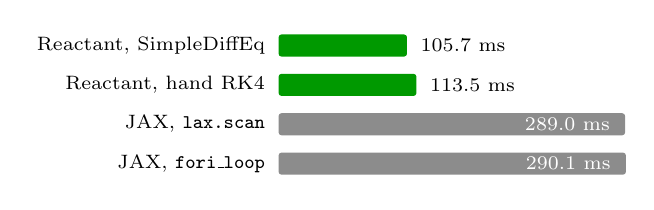
\begin{tikzpicture}[font=\scriptsize]
      % scale: 1 cm = 65 ms
      \node[anchor=east] at (0, 0)     {Reactant, SimpleDiffEq};
      \draw[fill=green!60!black, draw=none, rounded corners=1pt] (0.05,-0.14) rectangle (1.68, 0.14);
      \node[anchor=west] at (1.73, 0)  {105.7 ms};
      \node[anchor=east] at (0, -0.5)  {Reactant, hand RK4};
      \draw[fill=green!60!black, draw=none, rounded corners=1pt] (0.05,-0.64) rectangle (1.80,-0.36);
      \node[anchor=west] at (1.85,-0.5) {113.5 ms};
      \node[anchor=east] at (0, -1.0)  {JAX, \texttt{lax.scan}};
      \draw[fill=black!45, draw=none, rounded corners=1pt] (0.05,-1.14) rectangle (4.45,-0.86);
      \node[anchor=east, color=white] at (4.38,-1.0) {289.0 ms};
      \node[anchor=east] at (0, -1.5)  {JAX, \texttt{fori\_loop}};
      \draw[fill=black!45, draw=none, rounded corners=1pt] (0.05,-1.64) rectangle (4.46,-1.36);
      \node[anchor=east, color=white] at (4.39,-1.5) {290.1 ms};
    \end{tikzpicture}\\[0.7em]
    {\footnotesize\textbf{first call (compile)}}\\[0.3em]
    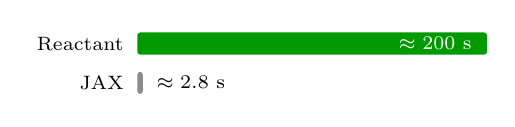
\begin{tikzpicture}[font=\scriptsize]
      % scale: 1 cm = 45 s
      \node[anchor=east] at (0, 0)     {Reactant};
      \draw[fill=green!60!black, draw=none, rounded corners=1pt] (0.05,-0.14) rectangle (4.49, 0.14);
      \node[anchor=east, color=white] at (4.42, 0)  {$\approx 200$ s};
      \node[anchor=east] at (0, -0.5)  {JAX};
      \draw[fill=black!45, draw=none, rounded corners=1pt] (0.05,-0.64) rectangle (0.12,-0.36);
      \node[anchor=west] at (0.17,-0.5) {$\approx 2.8$ s};
    \end{tikzpicture}
    \end{center}
  \end{column}
  \begin{column}{0.40\textwidth}
    {\footnotesize
    \textbf{Per step:} Reactant is ${\sim}2.7\times$ faster --- its \texttt{@trace for} lowers to a
    tighter XLA \texttt{while} than \texttt{scan}/\texttt{fori}.

    \vspace{0.5em}
    \textbf{First call:} JAX compiles ${\sim}70\times$ faster. Iterating on the model, you feel it;
    amortized over a training run, you don't.

    \vspace{0.5em}
    \textbf{SimpleDiffEq $\approx$ hand RK4:} same loss to 5 digits; the library integrator really is
    a free drop-in.}
  \end{column}
  \end{columns}

  \vspace{0.35em}
  {\footnotesize Loss $+$ gradient only, data on device, sync before stopping; median of 20 after
  warmup. RTX 4080 SUPER, Reactant 0.2.273, JAX 0.10.2 --- a statement about this program, not the
  two languages.}
\end{frame}

% ==================================================================
% Part 3 -- what the policies do
% ==================================================================

% ------------------------------------------------------------------
% Slide: Monod rollouts
% ------------------------------------------------------------------
\begin{frame}{What the learned policy does}
  \begin{center}
    \makebox[\textwidth][c]{%
      \includegraphics[width=1.08\textwidth,height=0.80\textheight,keepaspectratio]%
        {../paper/figures/monod_comparison.png}}
  \end{center}

  \vspace{0.2em}
  {\small Twenty draws of the true $(\mu_{\max}, K_s)$, the same twenty for each strategy.}
\end{frame}

% ------------------------------------------------------------------
% Slide: posteriors
% ------------------------------------------------------------------
\begin{frame}{Sharper posteriors}
  \begin{columns}[c]
  \begin{column}{0.42\textwidth}
    {\small
    \begin{tabular}{@{}lccc@{}}
      \toprule
      & sPCE & \multicolumn{2}{c}{RMSE ($\times 10^{3}$)} \\
      Design & (nats) & $\mu_{\max}$ & $K_s$ \\
      \midrule
      Adaptive policy   & $\mathbf{3.68}$ & $\mathbf{3.1}$ & $\mathbf{24.9}$ \\
      Static (BIM)      & $3.45$ & $4.4$ & $34.3$ \\
      Static (sPCE-opt) & $3.34$ & $5.6$ & $41.5$ \\
      \bottomrule
    \end{tabular}}

    \vspace{1.0em}
    \alert{Same number of measurements, about 30\% lower error.}
  \end{column}
  \begin{column}{0.55\textwidth}
    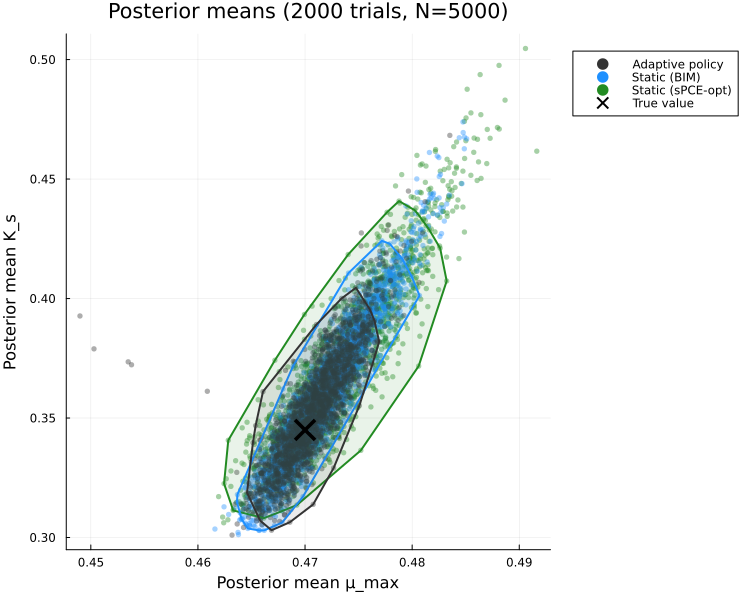
\includegraphics[width=\textwidth]{../paper/figures/monod_posterior.png}
  \end{column}
  \end{columns}
\end{frame}

% ------------------------------------------------------------------
% Slide: the design follows the data (Haldane)
% ------------------------------------------------------------------
\begin{frame}{Two runs, two different experiments}
  \begin{center}
    \makebox[\textwidth][c]{%
      \includegraphics[width=1.08\textwidth,height=0.72\textheight,keepaspectratio]%
        {../paper/figures/haldane_comparison.png}}
  \end{center}

  \vspace{0.2em}
  {\small Kinetics fixed; two values of the inhibition strength, twenty nuisance draws each.}

  \vspace{0.3em}
  \alert{The design adapts to the true parameters.}
\end{frame}

% ------------------------------------------------------------------
% Slide: DC motor
% ------------------------------------------------------------------
\begin{frame}{Real time: a DC motor on a 10\,ms clock}
  \begin{columns}[c]
  \begin{column}{0.55\textwidth}
    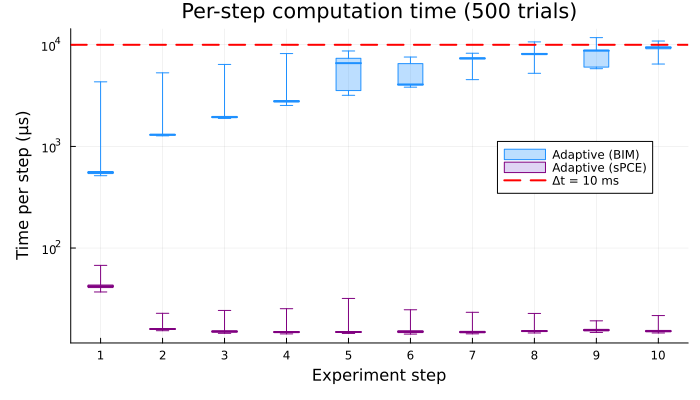
\includegraphics[width=\textwidth]{../paper/figures/dcmotor_timing.png}
  \end{column}
  \begin{column}{0.42\textwidth}
    \small
    \textbf{Adaptive (BIM)} --- re-optimized online. After every measurement: update the posterior,
    optimize the next voltage. All of it inside the $10$\,ms window.

    \vspace{0.9em}
    \textbf{Adaptive (sPCE)} --- the amortized policy. All of that happened offline, before the motor
    was switched on. Online, one forward pass.
  \end{column}
  \end{columns}

  \vspace{0.6em}
  \alert{Amortization is what makes adaptive design real-time.}
\end{frame}

% ------------------------------------------------------------------
% Slide: SciML integration
% ------------------------------------------------------------------
\begin{frame}[fragile]{Where this meets SciML}
  \small
  \begin{columns}[t]
  \begin{column}{0.52\textwidth}
    \textbf{SimpleDiffEq $+$ Reactant.}\ \
    We can use \texttt{SimpleDiffEq} via the low-level \texttt{init}/\texttt{step!}
    interface, needed for the \texttt{mincut} annotation:
\begin{lstlisting}[basicstyle=\smallcode]
prob  = ODEProblem(rhs, u, (0f0, dt), (θ, d))
integ = init(prob, SimpleRK4(); dt = dt_sub)
@trace mincut=true for _ in 1:n_substeps
    step!(integ)
end
\end{lstlisting}
    {\footnotesize A genuine drop-in: same loss as the hand-written RK4 to five digits,
    no runtime penalty.}

    \vspace{0.5em}
    \textbf{Adaptive solvers.}\ \
    For adaptive solvers this does not work: they pick the step count and $dt$ at run time,
    from the error estimate --- so when Reactant traces the program, there is no loop of
    known length to wrap the annotation around.
  \end{column}
  \begin{column}{0.44\textwidth}
    \textbf{Experimental: DiffEqReactant.jl.}
    \begin{itemize}\setlength{\itemsep}{0.3em}
      \item {\small A Tsit5 that is traceable by Reactant --- adaptivity expressed so the
            compiler can see it.}
      \item {\small Already trains a UDE with Lux $+$ Reactant $+$ Enzyme on the GPU.}
      \item {\small Very experimental; a deeper SciML integration is the goal.}
    \end{itemize}

    \vspace{0.5em}
    {\scriptsize \texttt{github.com/SebastianM-C/DiffEqReactant.jl}}
  \end{column}
  \end{columns}

  \vspace{0.5em}
  \alert{Fixed-step SciML solvers drop in today; traceable adaptive solvers are the next step.}
\end{frame}

% ------------------------------------------------------------------
% Slide: code and paper
% ------------------------------------------------------------------
\begin{frame}{Code and paper}
  \begin{columns}[c]
  \begin{column}{0.38\textwidth}
    \begin{center}
      \qrcode[height=3.4cm]{https://github.com/arno-papers/CDC2026}
    \end{center}
  \end{column}
  \begin{column}{0.58\textwidth}
    \small
    \texttt{github.com/arno-papers/CDC2026}

    \vspace{1.0em}
    Paper: \texttt{arXiv:2603.16146}
  \end{column}
  \end{columns}

  \vspace{1.0em}
  {\footnotesize The resources and services used in this work were provided by the VSC (Flemish
  Supercomputer Center), funded by the Research Foundation -- Flanders (FWO) and the Flemish Government.}
\end{frame}

\end{document}
